\documentclass[12pt,oneside]{amsart}
\usepackage[margin=1in]{geometry}
\usepackage{amsmath}
\usepackage{amsthm}
\usepackage{amsfonts}
\usepackage{amssymb}
\usepackage{stmaryrd}
\usepackage[hidelinks]{hyperref}
\usepackage{tikz}
\usetikzlibrary{cd,tikzmark}
\usepackage{mathrsfs}
\usepackage{cancel}
\usepackage{graphicx}
\usepackage{xcolor,colortbl}
\usepackage{multirow}
\usepackage{caption}
\usepackage{pgfplots}
\pgfplotsset{width=13cm,compat=1.9}
\graphicspath{ {./images/} }

\newenvironment{nouppercase}{%
  \let\uppercase\relax%
  \renewcommand{\uppercasenonmath}[1]{}}{}

% THEOREMS ------------------------------------------------------

\numberwithin{equation}{section}
\numberwithin{figure}{section}

\theoremstyle{plain}
\newtheorem{thm}[equation]{Theorem}
\newtheorem*{FundClaim*}{Fundamental Claim}
\newtheorem{lemma}[equation]{Lemma}
\newtheorem{cor}[equation]{Corollary}
\newtheorem{prop}[equation]{Proposition}
\newtheorem{example}[equation]{Example}
\newtheorem{prob}{Problem}

\theoremstyle{definition}
\newtheorem{definition}[equation]{Definition}
\newtheorem{question}[equation]{Question}
\newtheorem{remark}[equation]{Remark}


% MATH -----------------------------------------------------------
\newcommand{\Q}{\ensuremath \mathbb{Q}}
\newcommand{\R}{\ensuremath \mathbb{R}}
\newcommand{\C}{\ensuremath \mathbb{C}}
\newcommand{\Z}{\ensuremath \mathbb{Z}}
\newcommand{\N}{\ensuremath \mathbb{N}}
\newcommand{\M}{\ensuremath \mathbb{M}}
\newcommand{\F}{\ensuremath \mathbb{F}}
\newcommand{\Ord}{\text{Ord}}

\newcommand{\lxor}{\underline{\lor}}
\newcommand{\lnor}{\overline{\lor}}
\newcommand{\lnand}{\overline{\land}}
\newcommand{\dom}[1]{\text{dom}(#1)}
\newcommand{\ran}[1]{\text{ran}(#1)}
\newcommand{\rref}[1]{#1^\text{ref}}
\newcommand{\rsym}[1]{#1^\text{sym}}
\newcommand{\rtran}[1]{#1^\text{tran}}
\newcommand{\rirref}[1]{#1^\text{irref}}
\newcommand{\rasym}[1]{#1^\text{asym}}
\newcommand{\rantisym}[1]{#1^\text{antisym}}
\newcommand{\rintran}[1]{#1^\text{intran}}
\newcommand{\ldef}{\text{iff}_\text{def}}
\newcommand{\lub}[1]{\text{lub}_#1}
\newcommand{\glb}[1]{\text{glb}_#1}
\newcommand{\canon}[1]{#1_{\text{canon}}}
\newcommand{\pset}[2][]{\mathscr{P}^{#1}(#2)}
\newcommand{\fset}[2][]{\mathcal{F}^{#1}(#2)}
\newcommand{\restrict}[2]{#1\mid_{#2}}
\newcommand{\ceil}[1]{\ensuremath \lceil #1 \rceil}
\newcommand{\floor}[1]{\ensuremath \lfloor #1 \rfloor}

\DeclareMathOperator{\vspan}{span}
\makeatletter
\renewcommand*\env@matrix[1][*\c@MaxMatrixCols c]{%
  \hskip -\arraycolsep
  \let\@ifnextchar\new@ifnextchar
  \array{#1}}
\makeatother

\title{HW 2}
\author{Drew Morris}
\date{September 18th 2023}

\begin{document}

\maketitle

\renewcommand{\arraystretch}{1.5}

\begin{prob}
  Solve the following constrained maximization problem using simplex. \\
  \begin{center}\begin{tabular}{|ccccccccc|}
    \hline
    $6x_0$ & $+$ & $8x_1$ & $+$ & $5x_2$ & $+$ & $9x_3$ & $=$ & $\xi$ \\
    \hline
    $2x_0$ & $+$ & $x_1$ & $+$ & $x_2$ & $+$ & $3x_3$ & $\leq$ & $5$ \\
    $x_0$ & $+$ & $3x_1$ & $+$ & $x_2$ & $+$ & $2x_3$ & $\leq$ & $3$ \\
    $x_0$ & , & $x_1$ & , & $x_2$ & , & $x_3$ & $\geq$ & $0$ \\
    \hline
  \end{tabular}\end{center}
\end{prob}
Observe. \\
\begin{center}\begin{tabular}{ccccc}
  \begin{tabular}{|ccccccccccc|}
  \hline
  $\xi$ & $=$ & $0$ & $+$ & $6x_0$ & $+$ & $8x_1$ & $+$ & $5x_2$ & $+$ & $9x_3$ \\
  \hline
  $y_0$ & $=$ & $5$ & $-$ & $2x_0$ & $-$ & $x_1$  & $-$ & $x_2$  & $-$ & $3x_3$ \\
  $y_1$ & $=$ & $3$ & $-$ & $x_0$  & $-$ & $3x_1$ & $-$ & $x_2$  & $-$ & $2x_3$ \\
  \hline
\end{tabular} & $\to$ & $x_3 = \frac{3}{2}$ & $\to$ \\
\begin{tabular}{|ccccccccccc|}
  \hline
  $\xi$ & $=$ & $\frac{27}{2}$ & $+$ & $\frac{3}{2}x_0$ & $-$ & $\frac{11}{2}x_1$ & $+$ & $\frac{1}{2}x_2$ & $-$ & $\frac{9}{2}y_1$ \\
  \hline
  $y_0$ & $=$ & $\frac{1}{2}$  & $-$ & $\frac{1}{2}x_0$ & $+$ & $\frac{7}{2}x_1$ & $+$ & $\frac{1}{2}x_2$ & $+$ & $\frac{3}{2}y_1$ \\
  $x_3$ & $=$ & $\frac{3}{2}$  & $-$ & $\frac{1}{2}x_0$ & $-$ & $\frac{3}{2}x_1$ & $-$ & $\frac{1}{2}x_2$ & $-$ & $\frac{1}{2}y_1$ \\
  \hline
\end{tabular} & $\to$ & $x_0 = 1$ & $\to$ \\
\begin{tabular}{|ccccccccccc|}
  \hline
  $\xi$ & $=$ & $15$ & $-$ & $3y_0$ & $+$ & $5x_1$ & $+$ & $2x_2$ & $+$ & $0y_1$ \\
  \hline
  $x_0$ & $=$ & $1$  & $-$ & $2y_0$ & $+$ & $7x_1$ & $+$ & $x_2$  & $+$ & $3y_1$ \\
  $x_3$ & $=$ & $1$  & $+$ & $y_0$  & $-$ & $5x_1$ & $-$ & $x_2$  & $-$ & $2y_1$ \\
  \hline
\end{tabular} & $\to$ & $x_1 = \frac{1}{5}$ & $\to$ \\
\begin{tabular}{|ccccccccccc|}
  \hline
  $\xi$ & $=$ & $16$           & $-$ & $2y_0$           & $-$ & $x_3$            & $+$ & $x_2$            & $-$ & $2y_1$ \\
  \hline
  $x_0$ & $=$ & $\frac{12}{5}$ & $-$ & $\frac{3}{5}y_0$ & $-$ & $\frac{7}{5}x_3$ & $-$ & $\frac{2}{5}x_2$ & $+$ & $\frac{1}{5}y_1$ \\
  $x_1$ & $=$ & $\frac{1}{5}$  & $+$ & $\frac{1}{5}y_0$ & $-$ & $\frac{1}{5}x_3$ & $-$ & $\frac{1}{5}x_2$ & $-$ & $\frac{2}{5}y_1$ \\
  \hline
\end{tabular} & $\to$ & $x_2 = 1$ & $\to$ \\
\begin{tabular}{|ccccccccccc|}
  \hline
  $\xi$ & $=$ & $17$ & $-$ & $y_0$ & $-$ & $2x_3$ & $-$ & $5x_1$ & $-$ & $4y_1$ \\
  \hline
  $x_0$ & $=$ & $2$  & $-$ & $y_0$ & $-$ & $x_3$  & $+$ & $2x_1$ & $+$ & $y_1$ \\
  $x_2$ & $=$ & $1$  & $+$ & $y_0$ & $-$ & $x_3$  & $-$ & $5x_1$ & $-$ & $2y_1$ \\
  \hline
\end{tabular} & $\to$ & \multicolumn{3}{c}{$\xi = 17$} \\
\end{tabular}\end{center} \pagebreak

\begin{prob}
Solve the following constrained maximization problem using simplex. \\
\begin{center}\begin{tabular}{|ccccc|}
  \hline
  $3x_0$ & $+$ & $2x_1$ & $=$    & $\xi$ \\
  \hline
  $x_0$  & $-$ & $2x_1$ & $\leq$ & $1$   \\
  $x_0$  & $-$ & $x_1$  & $\leq$ & $2$   \\
  $2x_0$ & $-$ & $x_1$  & $\leq$ & $6$   \\
  $x_0$  & $+$ & $0x_1$ & $\leq$ & $5$   \\
  $2x_0$ & $+$ & $x_1$  & $\leq$ & $16$  \\
  $x_0$  & $+$ & $x_1$  & $\leq$ & $12$  \\
  $x_0$  & $+$ & $2x_1$ & $\leq$ & $21$  \\
  $0x_0$ & $+$ & $x_2$  & $\leq$ & $10$  \\
  $x_0$  & ,   & $x_1$  & $\geq$ & $0$   \\
  \hline
\end{tabular}\end{center}
\end{prob}
Observe. \\
\begin{center}\begin{tabular}{ccccc}
\begin{tabular}{|ccccccc|}
\hline
$\xi$ & $=$ & $0$  & $+$ & $3x_0$ & $+$ & $2x_1$ \\
\hline
$y_0$ & $=$ & $1$  & $-$ & $x_0$  & $+$ & $2x_1$ \\
$y_1$ & $=$ & $2$  & $-$ & $x_0$  & $+$ & $x_1$  \\
$y_2$ & $=$ & $6$  & $-$ & $2x_0$ & $+$ & $x_1$  \\
$y_3$ & $=$ & $5$  & $-$ & $x_0$  & $+$ & $0x_1$ \\
$y_4$ & $=$ & $16$ & $-$ & $2x_0$ & $-$ & $x_1$  \\
$y_5$ & $=$ & $12$ & $-$ & $x_0$  & $-$ & $x_1$  \\
$y_6$ & $=$ & $21$ & $-$ & $x_0$  & $-$ & $2x_1$ \\
$y_7$ & $=$ & $10$ & $+$ & $0x_0$ & $-$ & $x_1$  \\
\hline
\end{tabular} & $\to$ & $x_0 = 1$ & $\to$ \\
\begin{tabular}{|ccccccc|}
\hline
$\xi$ & $=$ & $3$  & $-$ & $3y_0$ & $+$ & $8x_1$ \\
\hline
$x_0$ & $=$ & $1$  & $-$ & $y_0$  & $+$ & $2x_1$ \\
$y_1$ & $=$ & $1$  & $+$ & $y_0$  & $-$ & $x_1$  \\
$y_2$ & $=$ & $4$  & $+$ & $2y_0$ & $-$ & $3x_1$ \\
$y_3$ & $=$ & $4$  & $+$ & $y_0$  & $-$ & $2x_1$ \\
$y_4$ & $=$ & $14$ & $+$ & $2y_0$ & $-$ & $5x_1$ \\
$y_5$ & $=$ & $11$ & $+$ & $y_0$  & $-$ & $3x_1$ \\
$y_6$ & $=$ & $20$ & $+$ & $y_0$  & $-$ & $4x_1$ \\
$y_7$ & $=$ & $10$ & $+$ & $0y_0$ & $-$ & $x_1$  \\
\hline
\end{tabular} & $\to$ & $x_1 = 1$ & $\to$ \\
\end{tabular}\end{center}\pagebreak\begin{center}\begin{tabular}{ccccc}
\begin{tabular}{|ccccccc|}
\hline
$\xi$ & $=$ & $11$ & $+$ & $5y_0$ & $-$ & $8y_1$ \\
\hline
$x_0$ & $=$ & $3$  & $+$ & $y_0$  & $-$ & $2y_1$ \\
$x_1$ & $=$ & $1$  & $+$ & $y_0$  & $-$ & $y_1$  \\
$y_2$ & $=$ & $1$  & $-$ & $y_0$  & $+$ & $3y_1$ \\
$y_3$ & $=$ & $2$  & $-$ & $y_0$  & $+$ & $2y_1$ \\
$y_4$ & $=$ & $9$  & $-$ & $3y_0$ & $+$ & $5y_1$ \\
$y_5$ & $=$ & $8$  & $-$ & $2y_0$ & $+$ & $3y_1$ \\
$y_6$ & $=$ & $16$ & $-$ & $3y_0$ & $+$ & $4y_1$ \\
$y_7$ & $=$ & $9$  & $-$ & $y_0$  & $+$ & $y_1$  \\
\hline
\end{tabular} & $\to$ & $y_0 = 1$ & $\to$ \\
\begin{tabular}{|ccccccc|}
\hline
$\xi$ & $=$ & $16$ & $-$ & $5y_2$ & $+$ & $7y_1$ \\
\hline
$x_0$ & $=$ & $4$  & $-$ & $y_2$  & $+$ & $y_1$  \\
$x_1$ & $=$ & $2$  & $-$ & $y_2$  & $+$ & $2y_1$ \\
$y_0$ & $=$ & $1$  & $-$ & $y_2$  & $+$ & $3y_1$ \\
$y_3$ & $=$ & $1$  & $+$ & $y_2$  & $-$ & $y_1$  \\
$y_4$ & $=$ & $6$  & $+$ & $3y_2$ & $-$ & $4y_1$ \\
$y_5$ & $=$ & $6$  & $+$ & $2y_2$ & $-$ & $3y_1$ \\
$y_6$ & $=$ & $13$ & $+$ & $3y_2$ & $-$ & $5y_1$ \\
$y_7$ & $=$ & $8$  & $+$ & $y_2$  & $-$ & $2y_1$ \\
\hline
\end{tabular} & $\to$ & $y_1 = 1$ & $\to$ \\
\begin{tabular}{|ccccccc|}
\hline
$\xi$ & $=$ & $23$ & $+$ & $2y_2$ & $-$ & $7y_3$ \\
\hline
$x_0$ & $=$ & $5$  & $+$ & $0y_2$ & $-$ & $y_3$  \\
$x_1$ & $=$ & $4$  & $+$ & $y_2$  & $-$ & $2y_3$ \\
$y_0$ & $=$ & $4$  & $+$ & $2y_2$ & $-$ & $3y_3$ \\
$y_1$ & $=$ & $1$  & $+$ & $y_2$  & $-$ & $y_3$  \\
$y_4$ & $=$ & $2$  & $-$ & $y_2$  & $+$ & $4y_3$ \\
$y_5$ & $=$ & $3$  & $-$ & $y_2$  & $+$ & $3y_3$ \\
$y_6$ & $=$ & $8$  & $-$ & $2y_2$ & $+$ & $5y_3$ \\
$y_7$ & $=$ & $6$  & $-$ & $y_2$  & $+$ & $2y_3$ \\
\hline
\end{tabular} & $\to$ & $y_2 = 2$ & $\to$ \\
\end{tabular}\end{center}\pagebreak\begin{center}\begin{tabular}{ccccc}\begin{tabular}{|ccccccc|}
\hline
$\xi$ & $=$ & $27$ & $-$ & $2y_4$ & $+$ & $y_3$  \\
\hline
$x_0$ & $=$ & $5$  & $+$ & $0y_4$ & $-$ & $y_3$  \\
$x_1$ & $=$ & $6$  & $-$ & $y_4$  & $+$ & $2y_3$ \\
$y_0$ & $=$ & $8$  & $-$ & $2y_4$ & $+$ & $5y_3$ \\
$y_1$ & $=$ & $3$  & $-$ & $y_4$  & $+$ & $3y_3$ \\
$y_2$ & $=$ & $2$  & $-$ & $y_4$  & $+$ & $4y_3$ \\
$y_5$ & $=$ & $1$  & $+$ & $y_4$  & $-$ & $y_3$  \\
$y_6$ & $=$ & $4$  & $+$ & $2y_4$ & $-$ & $3y_3$ \\
$y_7$ & $=$ & $4$  & $+$ & $y_4$  & $-$ & $2y_3$ \\
\hline
\end{tabular} & $\to$ & $y_3 = 1$ & $\to$ \\
\begin{tabular}{|ccccccc|}
\hline
$\xi$ & $=$ & $28$ & $-$ & $y_4$  & $-$ & $y_5$  \\
\hline
$x_0$ & $=$ & $4$  & $-$ & $y_4$  & $+$ & $y_5$  \\
$x_1$ & $=$ & $8$  & $+$ & $y_4$  & $-$ & $2y_5$ \\
$y_0$ & $=$ & $13$ & $+$ & $3y_4$ & $-$ & $5y_5$ \\
$y_1$ & $=$ & $6$  & $+$ & $2y_4$ & $-$ & $3y_5$ \\
$y_2$ & $=$ & $6$  & $+$ & $3y_4$ & $-$ & $4y_5$ \\
$y_3$ & $=$ & $1$  & $+$ & $y_4$  & $-$ & $y_5$  \\
$y_6$ & $=$ & $1$  & $-$ & $y_4$  & $+$ & $3y_5$ \\
$y_7$ & $=$ & $2$  & $-$ & $y_4$  & $+$ & $2y_5$ \\
\hline
\end{tabular} & $\to$ & \multicolumn{3}{c}{$\xi = 28$} \\
\end{tabular}\end{center}
\pagebreak
\begin{prob}
Show that the following dictionary cannot be the optimal dictionary for any 
linear programming problem in which $y_0,y_1$ are the initial slack variables. \\
\begin{center}
\begin{tabular}{|ccccccc|}
  \hline
  $\xi$ & $=$ & $4$ & $-$ & $y_0$  & $-$ & $2x_1$ \\
  \hline
  $x_0$ & $=$ & $3$ & $+$ & $0y_0$ & $-$ & $2x_1$ \\
  $y_1$ & $=$ & $1$ & $+$ & $y_0$  & $-$ & $x_1$  \\
  \hline
\end{tabular}
\end{center}
\end{prob}
If $y_0$ were an initial slack variable then we'd see $0ky_0 = k3 - kx_0 - k2x_1$ 
where $k \in \R$ is some number such that $0k = 1$. No such number exists.

\begin{prob}
Graph the region of feasible solutions for $2.8$ and show the sequence of 
dictionary solutions.
\end{prob}
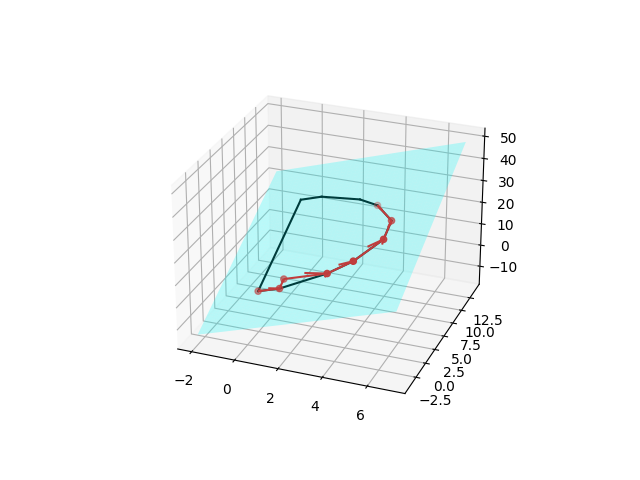
\includegraphics{Figure_1.png}
\pagebreak

\begin{prob}
Give an example showing that the variable that becomes basic in one iteration 
of the simplex method can become nonbasic in the next iteration.
\end{prob}
Consider the following problem. \\
\begin{center}\begin{tabular}{|ccccc|}
\hline
$3x_0$ & $+$ & $4x_1$ & $=$    & $\xi$ \\
\hline
$x_0$  & $+$ & $0x_1$ & $\leq$ & $4$   \\
$2x_0$ & $-$ & $x_1$  & $\leq$ & $6$   \\
$x_0$  & $+$ & $2x_1$ & $\leq$ & $2$   \\
$x_0$  & ,   & $x_1$  & $\geq$ & $0$   \\
\hline
\end{tabular}\end{center}
Observe. \\
\begin{center}\begin{tabular}{ccccc}
\begin{tabular}{|ccccccc|}
\hline
$\xi$ & $=$ & $0$ & $+$ & $3x_0$ & $+$ & $4x_1$ \\
\hline
$y_0$ & $=$ & $4$ & $-$ & $x_0$  & $+$ & $0x_1$ \\
$y_1$ & $=$ & $6$ & $-$ & $2x_0$ & $+$ & $x_1$  \\
$y_2$ & $=$ & $2$ & $-$ & $x_0$  & $-$ & $2x_1$ \\
\hline
\end{tabular} & $\to$ & $x_1 = 1$ & $\to$ & \\
\begin{tabular}{|ccccccc|}
\hline
$\xi$ & $=$ & $4$ & $+$ & $x_0$ & $-$ & $2y_2$ \\
\hline
$y_0$ & $=$ & $4$ & $-$ & $x_0$  & $+$ & $0y_2$ \\
$y_1$ & $=$ & $7$ & $-$ & $\frac{5}{2}x_0$ & $-$ & $\frac{1}{2}y_2$ \\
$x_1$ & $=$ & $1$ & $-$ & $\frac{1}{2}x_0$ & $-$ & $\frac{1}{2}y_2$ \\
\hline
\end{tabular} & $\to$ & $x_0 = 2$ & $\to$ & \\
\begin{tabular}{|ccccccc|}
\hline
$\xi$ & $=$ & $6$ & $-$ & $2x_1$ & $-$ & $3y_2$ \\
\hline
$y_0$ & $=$ & $2$ & $+$ & $2x_1$ & $+$ & $y_2$  \\
$y_1$ & $=$ & $2$ & $+$ & $5x_1$ & $+$ & $2y_2$ \\
$x_0$ & $=$ & $2$ & $-$ & $2x_1$ & $-$ & $y_2$  \\
\hline
\end{tabular} & $\to$ & \multicolumn{3}{c}{$\xi = 6$} \\
\end{tabular}\end{center}
After the first iteration, $x_1$ became a basic variable. Then after the 
second iteration, $x_1$ became a nonbasic variable.
\begin{prob}
Show that the variable that becomes nonbasic in one iteration of the simplex 
method cannot become basic in the next iteration.
\end{prob}
As show in the example for the previous problem, we can see whenever a variable 
becomes nonbasic, its leading coefficient in the equation that we are attempting 
to maximize will be negative, thus it will not be a candidate for our next 
entering variable and as such cannot become a basic variable during the next 
iteration. \pagebreak
\begin{prob}
Suppose that a linear programming problem has the following property. Its initial 
dictionary is not degenerate and when solved by the simplex method there is 
never a tie for the choice of the leaving variable.
\begin{enumerate}
  \item Can such a problem have degenerate dictionaries? Explain.
  \item Can such a problem cycle? Explain.
\end{enumerate}
\end{prob}
\begin{enumerate}
  \item Such a problem cannot yield a degenerate dictionary because there are no 
    ties in selection which means a degenerate dictionary could only follow from 
    a pervious dictionary, of which there is none because the initial dictionary 
    is non-degenerate.
  \item Such a problem cannot cycle because of what is mentioned above. To cycle, 
    a problem would have to contain a series of iterations through which you 
    yield the dictionary that started with at the beginning of the cycle. Because
    we cannot create any additional degeneracies by the answer above, there is no 
    first degeneracy to begin a cycle of degeneracies.
\end{enumerate}

\end{document}
